\documentclass[11pt,letterpaper,twoside]{article}
\usepackage[english]{babel}
\usepackage{amssymb,amsmath}
\usepackage{fancyhdr}
\usepackage{graphicx}
\usepackage{wrapfig}

 \oddsidemargin  0in \evensidemargin 0in
 \topmargin   -0.25in \headheight 0.25in \headsep 0.25in
 \textwidth   6.5in \textheight 8.75in \marginparsep 0pt \marginparwidth 0pt
 \parskip 1ex  \parindent 0ex \footskip 20pt

\newfont{\bssten}{cmssbx10}
\newfont{\bssnine}{cmssbx10 scaled 900}

%%%%%%%%%%%%%%%%%%%%%%%
\newcommand{\whatizit}{Lecture 12: The Normal Distribution}
%%%%%%%%%%%%%%%%%%%%%%%


\pagestyle{fancy}  
\fancyhead{\bssnine STOR 155,  \whatizit}
\fancyhead[RE]{} \fancyhead[LO]{}
\fancyhead[LE]{\bssnine \thepage} \fancyhead[RO]{\bssnine \thepage}
\lfoot{} \cfoot{} \rfoot{}   


\newcommand{\var}{\mathrm{Var}}



\begin{document}



\thispagestyle{empty} \vspace*{-0.75in}

{\bssten STOR 155: Introduction to Data Models and Inference \hfill June 4, 2024 \\
Prof. Will Lassiter  \hfill Page 1 of \pageref{totalpag}}
\vspace{10pt}
\begin{center} {{\Large \bf \whatizit}} \end{center}

{\bf Continuous Random Variables} \vspace{6pt}

Recall: A {\bf continuous} random variable is ... \vspace{60pt}

Example: Test scores

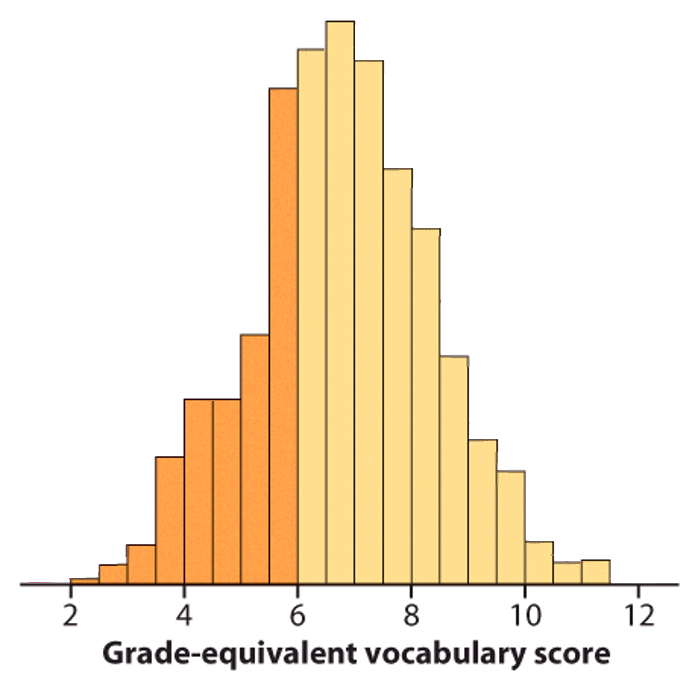
\includegraphics[scale=0.4]{images/histogram.png}

\vspace{20pt}

A different approach:

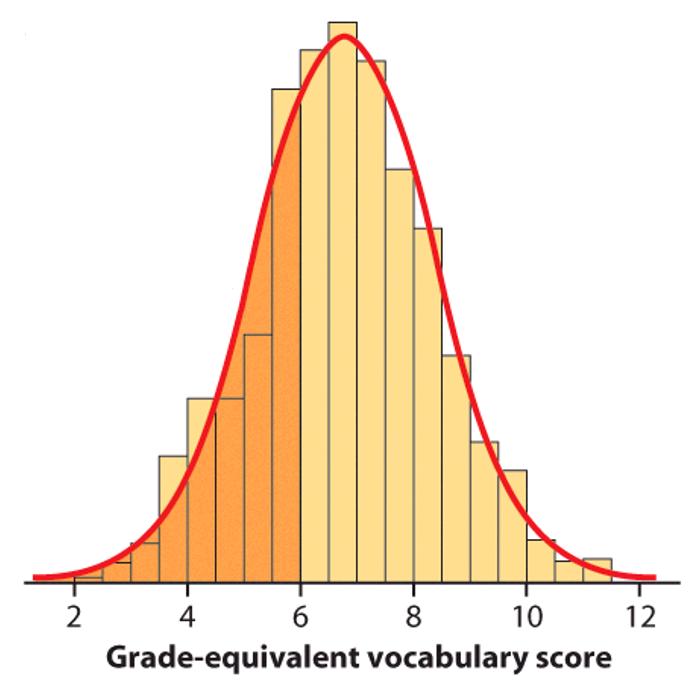
\includegraphics[scale=0.4]{images/histogram2.png}

\newpage

Definition: A {\bf density curve} is ... \vspace{100pt}

\begin{center}
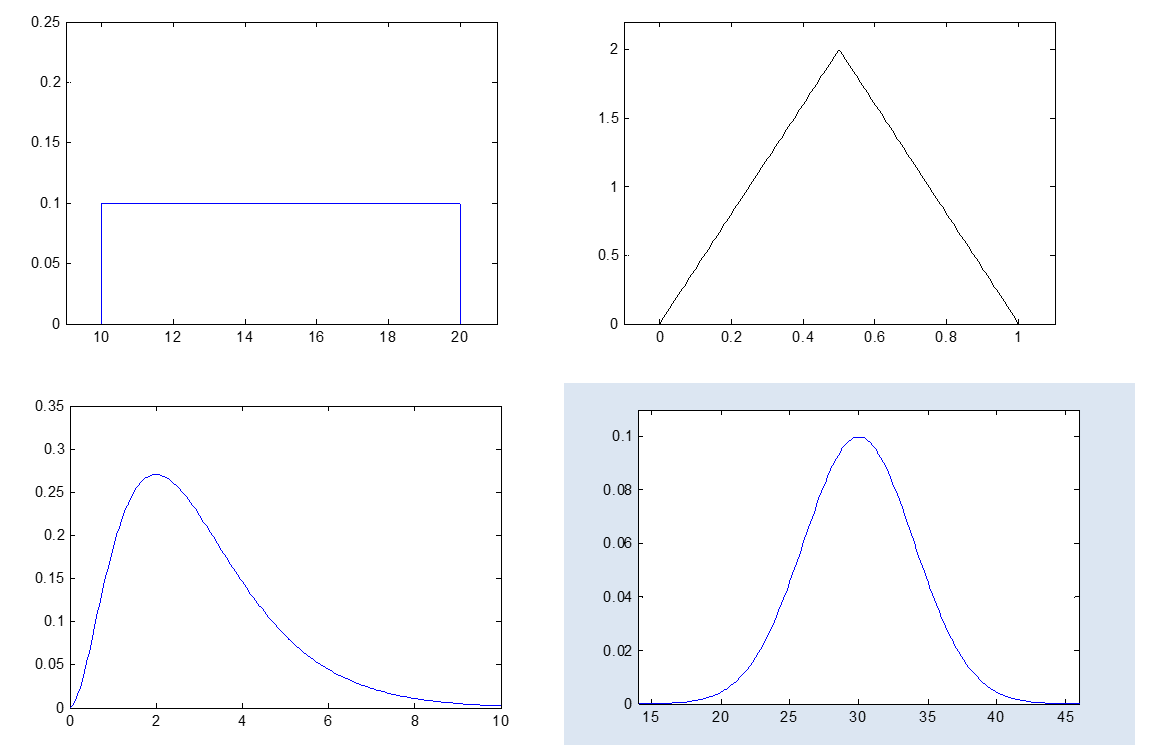
\includegraphics[scale=0.9]{images/densities.png}
\end{center}

Using a density curve to find proportions/probabilities \vspace{10pt}

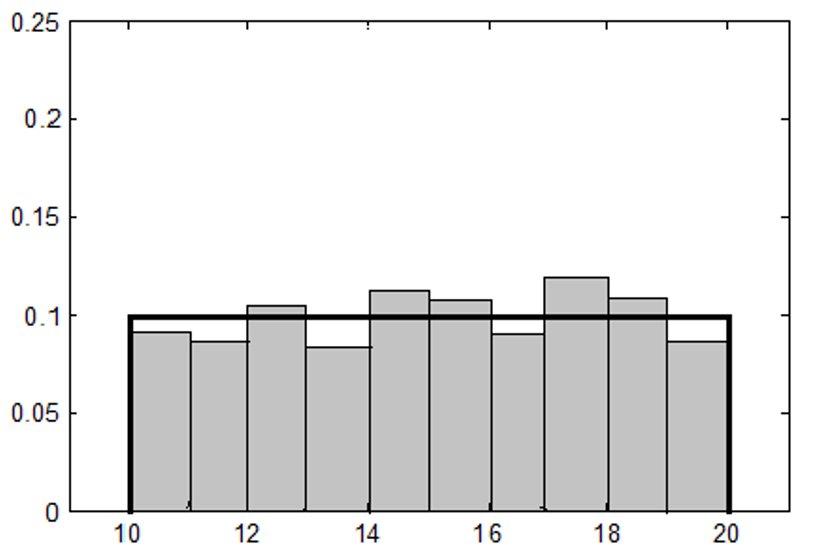
\includegraphics[width=8.0cm]{images/uniform.png}\hspace{10pt} 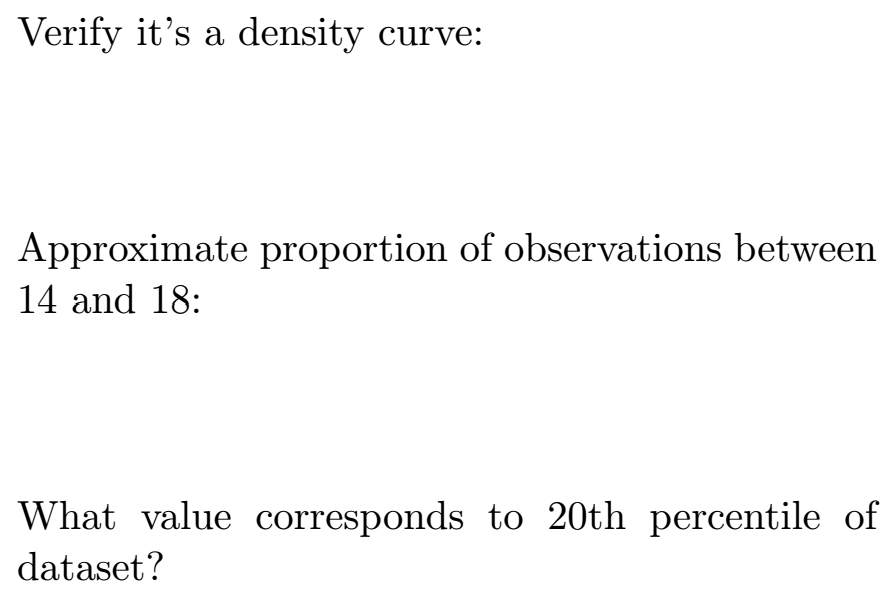
\includegraphics[scale=0.65]{images/questions.png}

\newpage

Another example: \vspace{6pt}

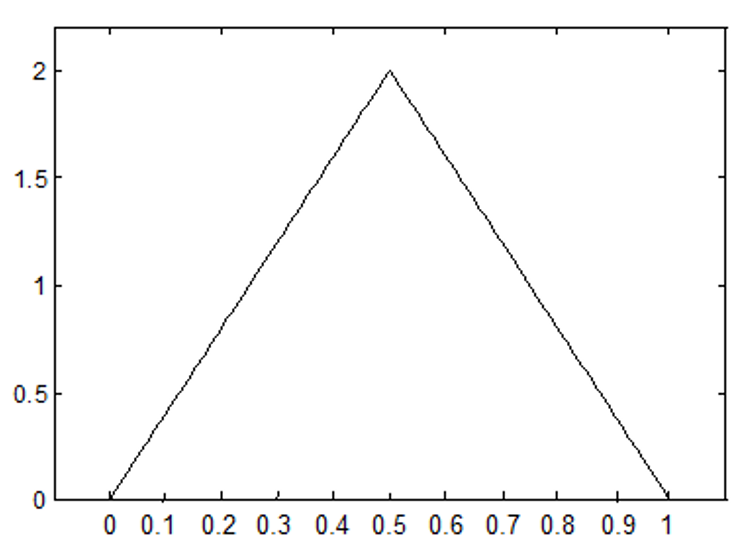
\includegraphics[scale=0.75]{images/triangular.png}\hspace{15pt} 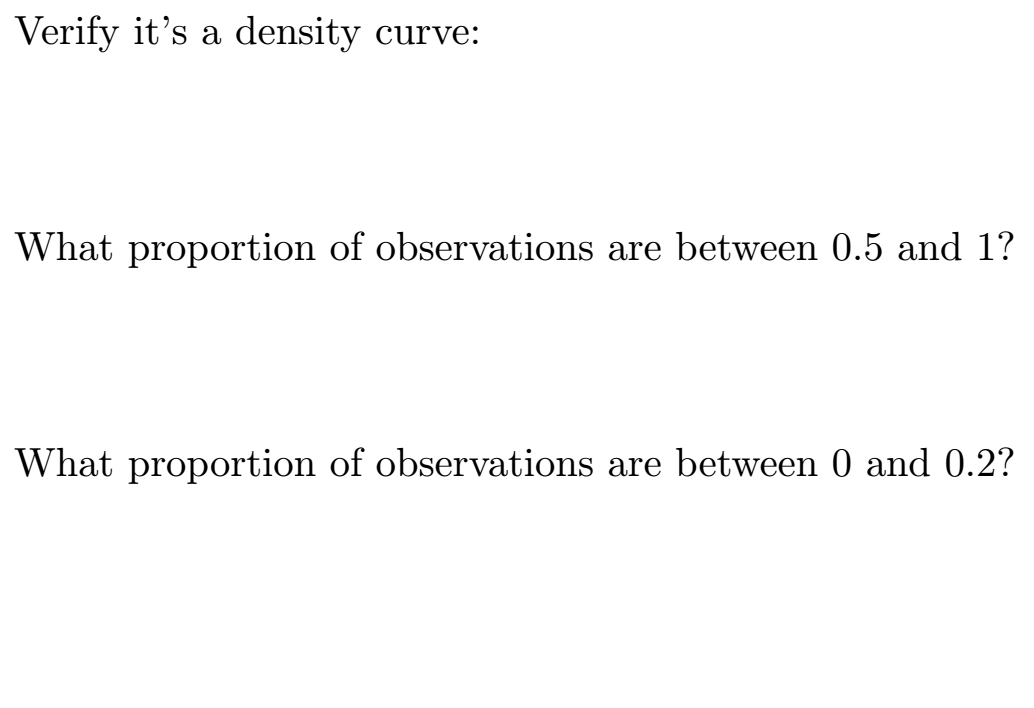
\includegraphics[scale=0.6]{images/questions2.png}

\vspace{10pt}

Approximating mean and median from a density curve:

\begin{center}
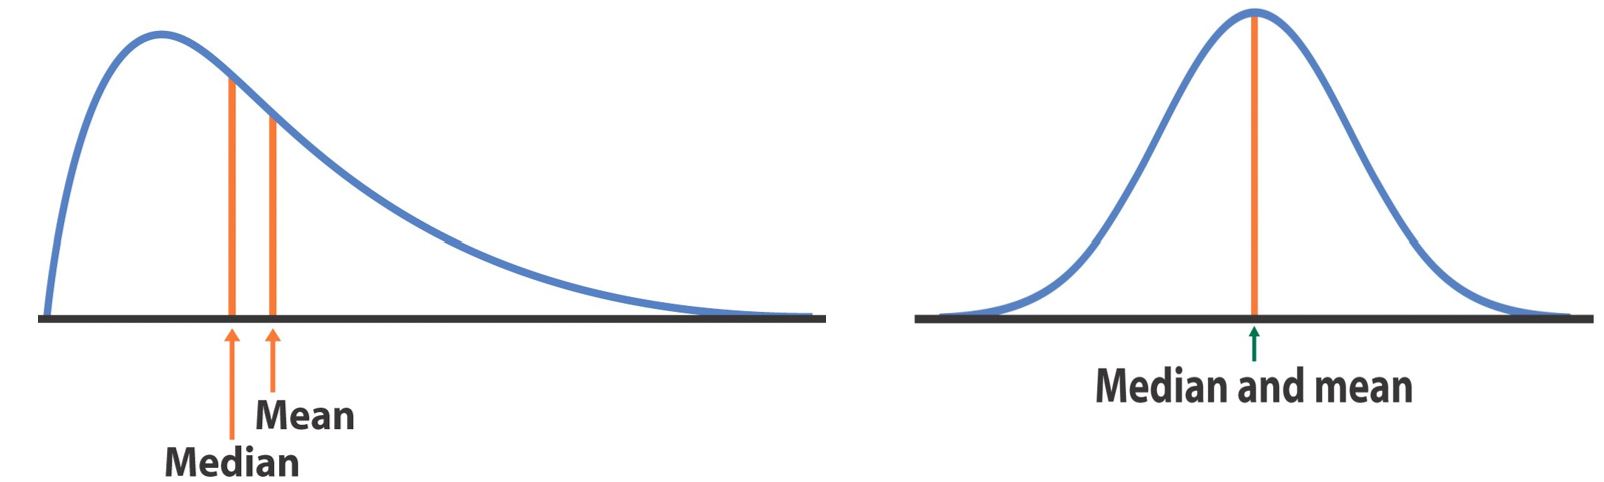
\includegraphics[scale=0.7]{images/meanmedian.png}
\end{center}

\vspace{100pt}

{\bf Normal Density Curves}

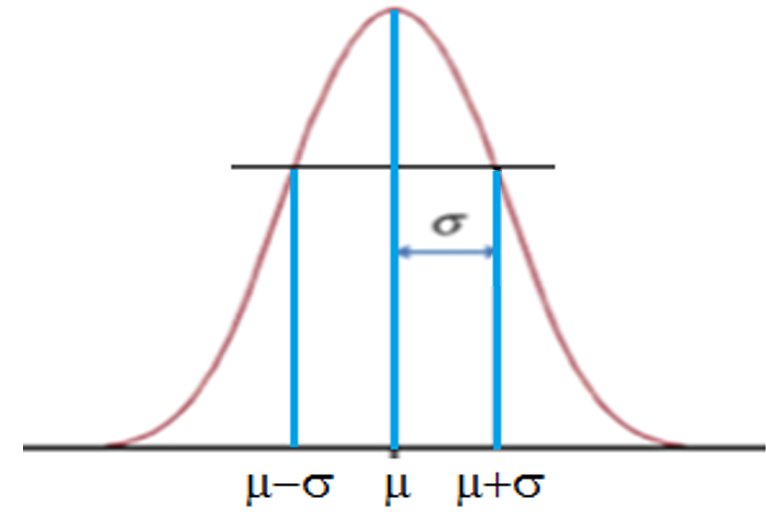
\includegraphics[scale=0.3]{images/inflection.png} \hspace{20pt}  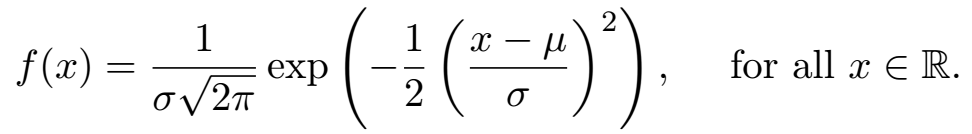
\includegraphics[scale=0.7]{images/normalfunction.png}

%\[ f(x)=\frac{1}{\sigma\sqrt{2\pi}}\exp\left(-\frac{1}{2}\left(\frac{x-\mu}{\sigma}\right)^2\right),\quad\mbox{ for all }x\in\mathbb{R}. \]

\newpage

Varying mean and standard deviation:

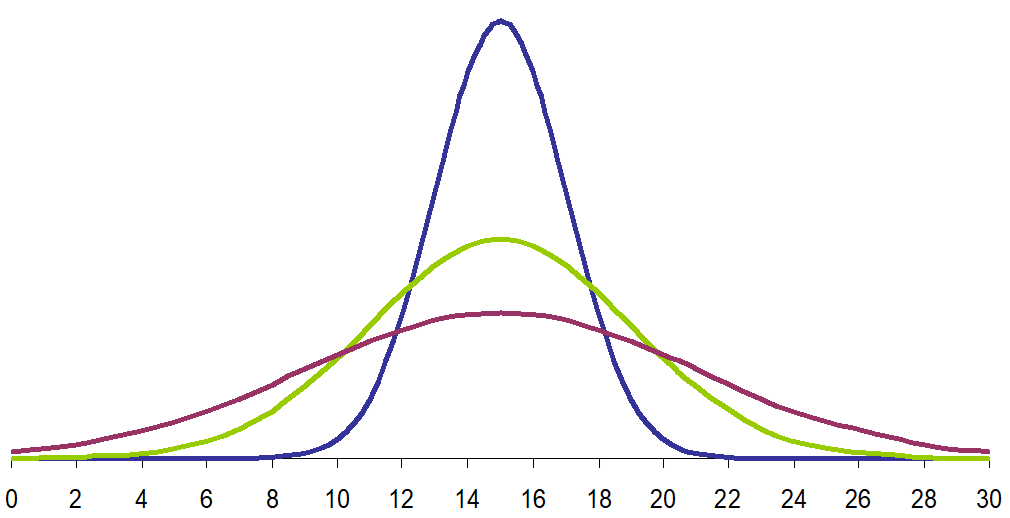
\includegraphics[scale=0.6]{images/stdev.png}\hspace{15pt} 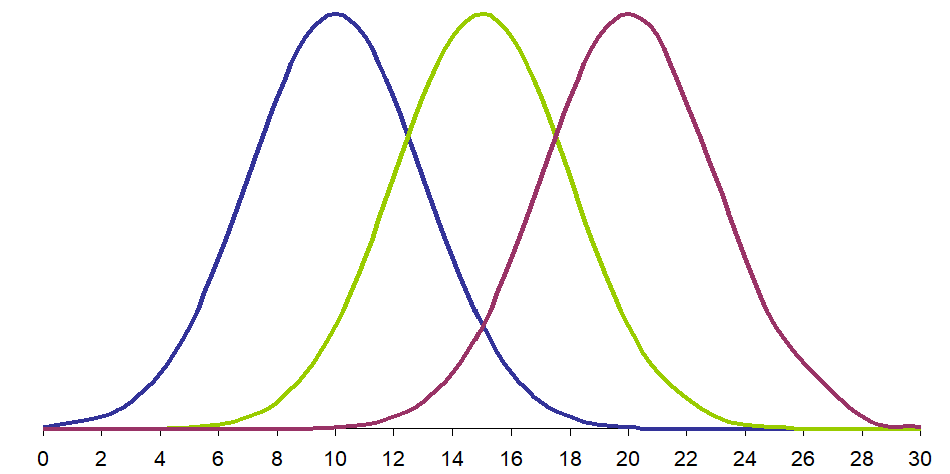
\includegraphics[scale=0.6]{images/mean.png}

\vspace{120pt}

The 68-95-99.7 Rule

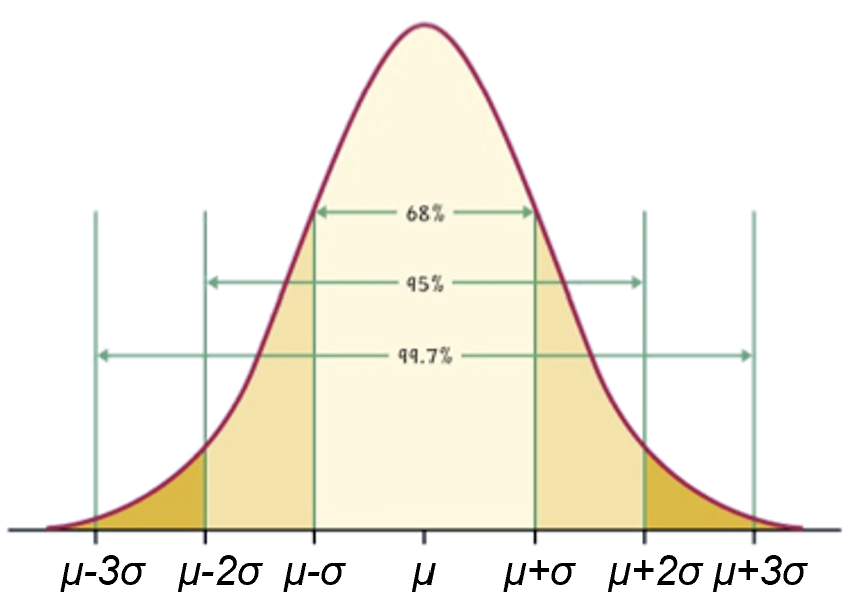
\includegraphics[scale=0.8]{images/68.png} \vspace{50pt}

Example: Heights of US women have an approximately normal distribution with mean 64.5 inches and standard deviation 2.5 inches.

\begin{itemize}

\item About 68\% of US women are between \_\_\_\_\_\_\_\_\_\_ and \_\_\_\_\_\_\_\_\_\_ inches tall. \vspace{10pt}

\item About 95\% of US women are between \_\_\_\_\_\_\_\_\_\_ and \_\_\_\_\_\_\_\_\_\_ inches tall. \vspace{10pt}

\item About 99.7\% of US women are between \_\_\_\_\_\_\_\_\_\_ and \_\_\_\_\_\_\_\_\_\_ inches tall.


\end{itemize}

\newpage

Example: 2.4 million people took the SAT in 2023. Scores were approximately normally distributed with mean $\mu = 1025$ and standard deviation $\sigma= 209$. Using the 68-95-99.7 rule...

\begin{itemize}

\item ... about \_\_\_\_\_\_\_\_\_\_\_\_\_\_\_\_\_\_\_\_\_\_ test takers scored between \_\_\_\_\_\_\_\_\_\_ and \_\_\_\_\_\_\_\_\_\_. \vspace{10pt}

\item ... about \_\_\_\_\_\_\_\_\_\_\_\_\_\_\_\_\_\_\_\_\_\_ test takers scored between \_\_\_\_\_\_\_\_\_\_ and \_\_\_\_\_\_\_\_\_\_. \vspace{10pt}

\item ... about \_\_\_\_\_\_\_\_\_\_\_\_\_\_\_\_\_\_\_\_\_\_ test takers scored between \_\_\_\_\_\_\_\_\_\_ and \_\_\_\_\_\_\_\_\_\_. \vspace{10pt}


\end{itemize}

The Standard Normal Density Curve

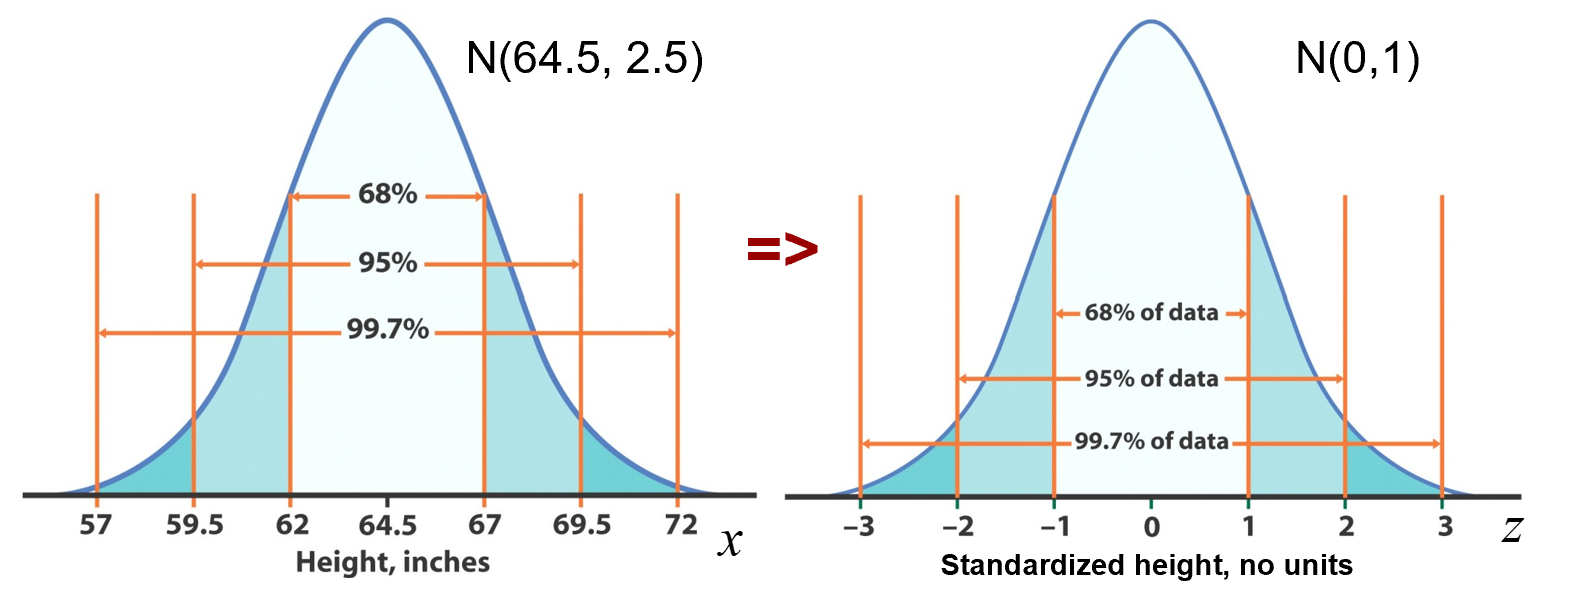
\includegraphics[scale=0.75]{images/standard.png}

\vspace{100pt}

{\bf $\mathbf{z}$-score}

\vspace{100pt}

Example: back to heights of US women

\newpage

Example: Prices of items at a big-box store are well-approximated by a normal distribution with mean \$20 and standard deviation \$5.

\begin{itemize}

\item Calculate the $z$-score for an item priced at \$10, then approximate the proportion of items priced below \$10. \vspace{60pt}

\item Approximate the proportion of items priced between \$10 and \$25. \vspace{60pt}

\item What proportion of items are priced higher than \$22.15?  \vspace{60pt}

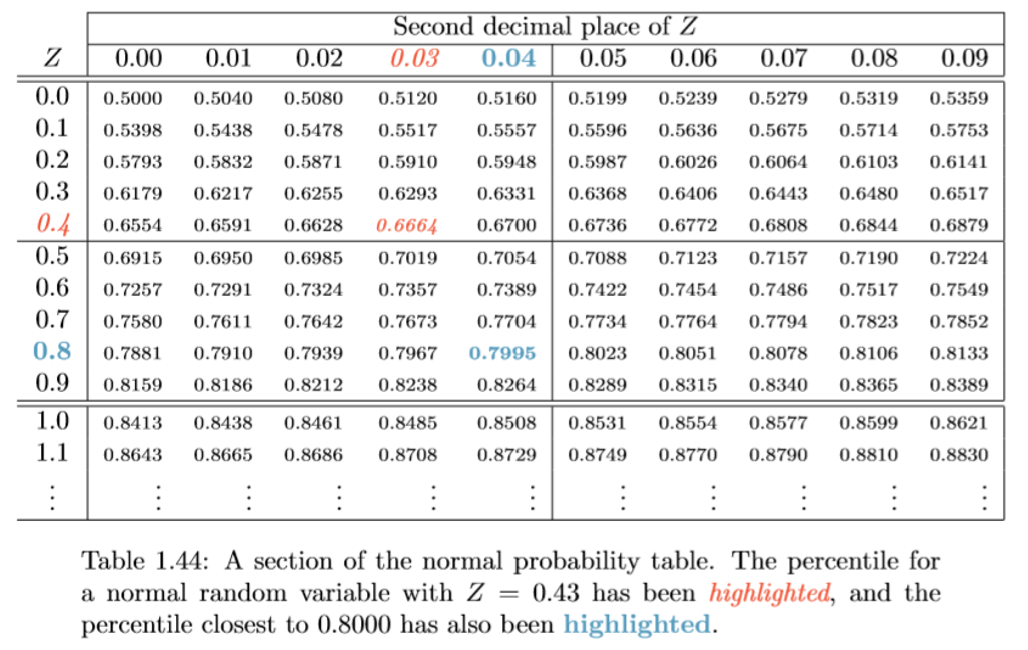
\includegraphics[scale=1.05]{images/ztable.png} \vspace{10pt}

\item What price corresponds to the $80^{\text{th}}$ percentile of prices of items sold in the store?

\end{itemize}

\newpage

Excel functions for calculating normal probabilities and percentiles:

\vspace{190pt}

Example: Back to the SAT: 2.4 million people took the SAT in 2023 and Scores were approximately normally distributed with mean $\mu = 1025$ and standard deviation $\sigma= 209$.

\begin{itemize}

\item What proportion of test-takers scored below 900? \vspace{60pt}

\item What proportion of test-takers scored between 900 and 1200? \vspace{60pt}

\item What score marks the top 5\% of all scores? \vspace{60pt}

\end{itemize}

More practice: Body temperatures of healthy humans are distributed nearly normally with mean $98.2^\circ$F and standard deviation $0.73^\circ$F. What is the cutoff for the highest 10\% of human body temperatures?

\begin{enumerate}

\item[(a)] $97.3^\circ$F

\item[(b)] $99.1^\circ$F

\item[(c)] $99.4^\circ$F

\item[(d)] $99.6^\circ$F

\end{enumerate}

\label{totalpag}
\end{document}
